\documentclass[a4paper,14pt,oneside,final]{extarticle}
\usepackage[top=2cm, bottom=2cm, left=3cm, right=1cm]{geometry}
\usepackage{scrextend}

\usepackage[T2A,T1]{fontenc}
\usepackage[ukrainian,russian,english]{babel}
\usepackage{tempora}
\usepackage{fontspec}
\setmainfont{tempora}

% Зачем: Отключает использование изменяемых межсловных пробелов.
% Почему: Так не принято делать в текстах на русском языке.
\frenchspacing

\usepackage{indentfirst}
\setlength{\parindent}{1.25cm}
\renewcommand{\baselinestretch}{1.5}

% Header
\usepackage{fancyhdr}
\pagestyle{fancy}
\fancyhead{}
\fancyfoot{}
\fancyhead[R]{\small \selectfont \thepage}
\renewcommand{\headrulewidth}{0pt}

% Captions
\usepackage{chngcntr}
\counterwithin{figure}{section}
\counterwithin{table}{section}
\usepackage[tableposition=top]{caption}
\usepackage{subcaption}
\DeclareCaptionLabelFormat{gostfigure}{Рисунок #2}
\DeclareCaptionLabelFormat{gosttable}{Таблиця #2}
\DeclareCaptionLabelSeparator{gost}{~---~}
\captionsetup{labelsep=gost}
\captionsetup[figure]{labelformat=gostfigure}
\captionsetup[table]{labelformat=gosttable}
\renewcommand{\thesubfigure}{\asbuk{subfigure}}

% Sections
\usepackage[explicit]{titlesec}
\newcommand{\sectionbreak}{\clearpage}

\titleformat{\section}
  {\centering}{\thesection \quad}{0pt}{\MakeUppercase{#1}}
\titleformat{\subsection}[block]
  {\bfseries}{\thesubsection \quad #1}{0cm}{}

\titlespacing{\section} {0cm}{0cm}{21pt}
\titlespacing{\subsection} {\parindent}{21pt}{0cm}
\titlespacing{\subsubsection} {\parindent}{0cm}{0cm}

% Lists
\usepackage{enumitem}
\renewcommand\labelitemi{--}
\setlist[itemize]{noitemsep, topsep=0pt, wide}
\setlist[enumerate]{noitemsep, topsep=0pt, wide, label=\arabic*}
\setlist[description]{labelsep=0pt, noitemsep, topsep=0pt, leftmargin=2\parindent, labelindent=\parindent, labelwidth=\parindent, font=\normalfont}

% Toc
\usepackage{tocloft}
\tocloftpagestyle{fancy}
\renewcommand{\cfttoctitlefont}{}
\setlength{\cftbeforesecskip}{0pt}
\renewcommand{\cftsecfont}{}
\renewcommand{\cftsecpagefont}{}
\renewcommand{\cftsecleader}{\cftdotfill{\cftdotsep}}

\usepackage{float}
\usepackage{pgfplots}
\usepackage{graphicx}
\usepackage{multirow}
\usepackage{amssymb,amsfonts,amsmath,amsthm}
\usepackage{csquotes}

\usepackage{listings}
\lstset{basicstyle=\footnotesize\ttfamily,breaklines=true}
\lstset{language=Matlab}

\usepackage[
	backend=biber,
	sorting=none,
	language=auto,
	autolang=other
]{biblatex}
\DeclareFieldFormat{labelnumberwidth}{#1}

\lstdefinelanguage{Python}{
  keywords={and, break, class, continue, def, yield, del, elif, else, except, exec, finally, for, from, global, if, import, in, lambda, not, or, pass, print, raise, return, try, while, assert, with},
  keywordstyle=\color{NavyBlue}\bfseries,
  ndkeywords={True, False},
  ndkeywordstyle=\color{BurntOrange}\bfseries,
  emph={as},
  emphstyle={\color{OrangeRed}},
  identifierstyle=\color{black},
  sensitive=true,
  commentstyle=\color{gray}\ttfamily,
  comment=[l]{\#},
  morecomment=[s]{/*}{*/},
  stringstyle=\color{ForestGreen}\ttfamily,
  morestring=[b]',
  morestring=[s]{"""*}{*"""},
}


\newcommand{\labnumber}{2} % second lab
\documentclass[a4paper,14pt,oneside,final]{extarticle}
\usepackage[top=2cm, bottom=2cm, left=3cm, right=1cm]{geometry}
\usepackage{scrextend}

\usepackage[T2A,T1]{fontenc}
\usepackage[ukrainian,russian,english]{babel}
\usepackage{tempora}
\usepackage{fontspec}
\setmainfont{tempora}

% Зачем: Отключает использование изменяемых межсловных пробелов.
% Почему: Так не принято делать в текстах на русском языке.
\frenchspacing

\usepackage{indentfirst}
\setlength{\parindent}{1.25cm}
\renewcommand{\baselinestretch}{1.5}

% Header
\usepackage{fancyhdr}
\pagestyle{fancy}
\fancyhead{}
\fancyfoot{}
\fancyhead[R]{\small \selectfont \thepage}
\renewcommand{\headrulewidth}{0pt}

% Captions
\usepackage{chngcntr}
\counterwithin{figure}{section}
\counterwithin{table}{section}
\usepackage[tableposition=top]{caption}
\usepackage{subcaption}
\DeclareCaptionLabelFormat{gostfigure}{Рисунок #2}
\DeclareCaptionLabelFormat{gosttable}{Таблиця #2}
\DeclareCaptionLabelSeparator{gost}{~---~}
\captionsetup{labelsep=gost}
\captionsetup[figure]{labelformat=gostfigure}
\captionsetup[table]{labelformat=gosttable}
\renewcommand{\thesubfigure}{\asbuk{subfigure}}

% Sections
\usepackage[explicit]{titlesec}
\newcommand{\sectionbreak}{\clearpage}

\titleformat{\section}
  {\centering}{\thesection \quad}{0pt}{\MakeUppercase{#1}}
\titleformat{\subsection}[block]
  {\bfseries}{\thesubsection \quad #1}{0cm}{}

\titlespacing{\section} {0cm}{0cm}{21pt}
\titlespacing{\subsection} {\parindent}{21pt}{0cm}
\titlespacing{\subsubsection} {\parindent}{0cm}{0cm}

% Lists
\usepackage{enumitem}
\renewcommand\labelitemi{--}
\setlist[itemize]{noitemsep, topsep=0pt, wide}
\setlist[enumerate]{noitemsep, topsep=0pt, wide, label=\arabic*}
\setlist[description]{labelsep=0pt, noitemsep, topsep=0pt, leftmargin=2\parindent, labelindent=\parindent, labelwidth=\parindent, font=\normalfont}

% Toc
\usepackage{tocloft}
\tocloftpagestyle{fancy}
\renewcommand{\cfttoctitlefont}{}
\setlength{\cftbeforesecskip}{0pt}
\renewcommand{\cftsecfont}{}
\renewcommand{\cftsecpagefont}{}
\renewcommand{\cftsecleader}{\cftdotfill{\cftdotsep}}

\newcommand{\khpistudentgroup}{КН-34г}
\newcommand{\khpistudentname}{Чепурний~А.~С.}

\newcommand{\khpidepartment}{Програмна інженерія та інформаційні технології управління}
\newcommand{\khpititlewhat}{
	Лабораторна робота №\labnumber \\
	з предмету <<Моделювання систем>>
}
\newcommand{\khpititlewho}{
	Виконав: \\
	\hspace*{\parindent} ст. групи \khpistudentgroup \\
	\hspace*{\parindent} \khpistudentname \\
	Перевірила: \\
	\hspace*{\parindent} ст. в. каф. ПІІТУ \\
	\hspace*{\parindent} Єршова~С.~І. \\
	\hspace*{\parindent} ас. каф. ПІІТУ \\
	\hspace*{\parindent} Литвинова~Ю.~С. \\
}



\graphicspath{{figures/}}

\begin{document}
\Ukrainian

\begin{titlepage}

\begin{center}
	МІНІСТЕРСТВО ОСВІТИ І НАУКИ УКРАЇНИ \\
	НАЦІОНАЛЬНИЙ ТЕХНІЧНИЙ УНІВЕРСИТЕТ \\
	«ХАРКІВСЬКИЙ ПОЛІТЕХНІЧНИЙ ІНСТИТУТ» \\[0.5cm]
	Кафедра <<\khpidepartment>> \\
\end{center}

\vspace{6cm}

\begin{center}
	\khpititlewhat
\end{center}

\vspace{3cm}

\begin{addmargin}[10cm]{0cm}
	\khpititlewho
\end{addmargin}

\vspace{\fill}

\begin{center}
	Харків \the\year
\end{center}

\end{titlepage}

\addtocounter{page}{1}

\section{Розробка інтелектуальної системи на мові CLIPS}
\subsubsection*{Мета}
Розробка інтелектуальної системи на мові CLIPS.
\subsubsection*{Постановка задач}
Вивчення технології пошуку вирішення завдань з урахуванням інтелектуальних принципів, на базі продукционной моделі знань, тобто моделі, заснованої на правилах, яка дозволяє представити знання у вигляді пропозицій типу <<Якщо, то>>, і набуття навичок їх практичної реалізації на мові CLIPS.

\begin{center}
    Варіант 3 --- CLIPS програма для онтології розробленої в Protege.
\end{center}

\subsection{Аналіз предметної області}
Предметною областю є управління медичними страховими договорами приєднання.

Метою створення онтології є керування створенням договорів страхування, вибір оптимальної програми страхування  

Глосарій предметної області:
\begin{enumerate}
  \item Страховик --- страхова компанія, яка надає послуги страхування. 
  \item Страхувальник --- фізична особа, яка уклала договір про страхування здоров'я та працездатності на свою користь.
  \item Страхова сума --- грошова сума, в межах якої страховик відповідно до умов договору страхування зобов'язаний здійснювати страхові виплати при настанні страхового випадку. 
  \item Страховий випадок --- подія, передбачена договором страхування, яка відбулася після набуття чинності договору страхування і з настанням якої виникає обов'язок страховика здійснити страхову виплату страхувальнику.
  \item Страховий ризик --- певна подія, на випадок якої проводиться страхування і яка має ознаки ймовірності та випадковості настання.
  \item Медичне страхування --- тип страхування від ризику витрат, пов'язаних із отриманням медичної допомоги.
  \item Договір приєднання --- договір, умови якого встановлені однією із сторін у формулярах або інших стандартних формах, який може бути укладений лише шляхом приєднання другої сторони до запропонованого договору в цілому. 
  \item Договір страхування --- договір приєднання медичного страхування. 
\end{enumerate}

При виникненні страхового випадку страховик гарантує оплату медичної допомоги, за рахунок накопичених страхувальниками коштів. 
Медичне страхування дозволяє гарантувати громадянину безкоштовне надання певного обсягу медичних послуг, при виникненні страхового випадку (порушення здоров'я), за наявності договору зі страховиком. 
Остання несе витрати з оплати випадку надання медичної допомоги, з моменту сплати громадянином першого внеску до відповідного фонду.

\subsection{Розробка моделі даних для обраної предметної області}
Згідно заданій предметній області була розроблена концептуальна модель бази даних, що зображена на рисунку~\ref{fig:er}.

\begin{figure}[H]
    \centering
        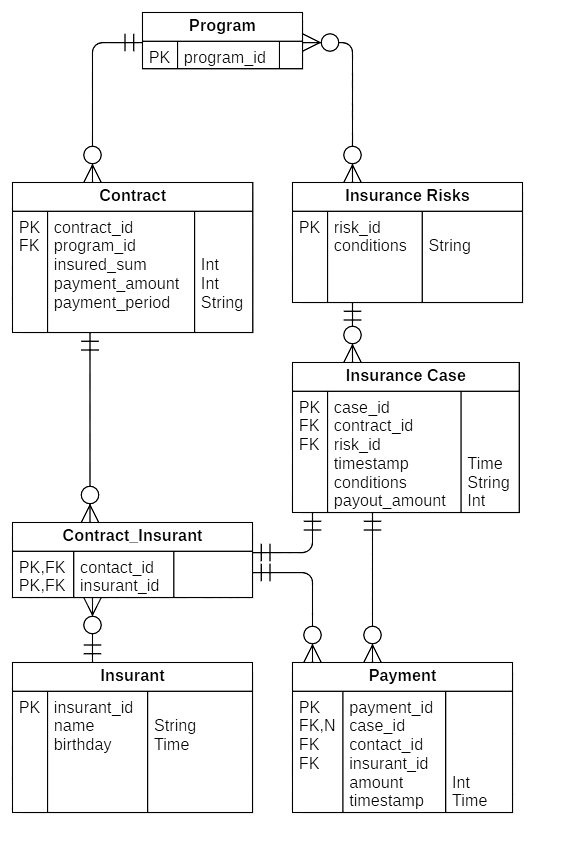
\includegraphics[width=0.6\linewidth]{er}
    \caption{Концептуальна модель бази даних}
    \label{fig:er}
\end{figure}

Перелік сутностей в моделі даних: 
\begin{itemize}
  \item \texttt{Program} --- страхова програма;
  \item \texttt{Contract} --- страховий договір приєднання;
  \item \texttt{Insurance Risks} --- страхові ризики;
  \item \texttt{Insurance Case} --- страховий випадок;
  \item \texttt{Insurant} --- страхувальник;
  \item \texttt{Payment} --- виплати.
\end{itemize}

\subsection{Розробка онтології для обраної предметної області}
Для обраної предметної області була розроблена онтологія згідно стандарту IDEF5. 
Діаграми стану, взаємозв'язку, композиціі та класифікації договору страхування представлені на рисунках~\ref{fig:idef_state}, \ref{fig:idef_relation}, \ref{fig:idef_composition}, \ref{fig:idef_classification}.

\begin{figure}[H]
    \centering
        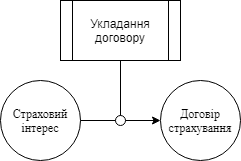
\includegraphics{idef_state}
    \caption{Діаграма стану укладання договору}
    \label{fig:idef_state}
\end{figure}

\begin{figure}[H]
    \centering
        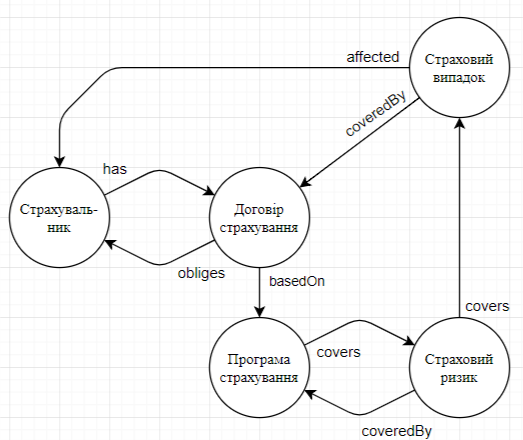
\includegraphics[width=0.7\linewidth]{idef_relation}
    \caption{Взаємозв'язок договору страхування}
    \label{fig:idef_relation}
\end{figure}

\begin{figure}[H]
    \centering
        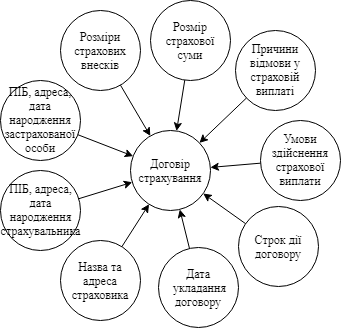
\includegraphics[width=0.6\linewidth]{idef_composition}
    \caption{Композиційна схема договору страхування}
    \label{fig:idef_composition}
\end{figure}

\begin{figure}[H]
    \centering
        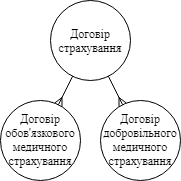
\includegraphics{idef_classification}
    \caption{Класифікація договорів страхування}
    \label{fig:idef_classification}
\end{figure}

\subsection{Сутності в Protege}
В результаті аналізу ПрО <<Управління страховими договорами>>, який був проведений, додалися наступні сутності (рисунок~\ref{fig:class_props}, рисунок~\ref{fig:data_props} та рисунок~\ref{fig:object_props}).

\begin{figure}[H]
    \centering
    \begin{subfigure}[b]{0.3\textwidth}
        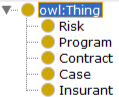
\includegraphics{class_props}
    \caption{Класи}
    \label{fig:class_props}
    \end{subfigure}
    ~
    \begin{subfigure}[b]{0.3\textwidth}
        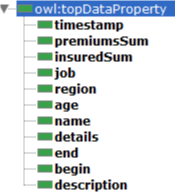
\includegraphics{data_props}
    \caption{Параметри даних}
    \label{fig:data_props}
    \end{subfigure}
    ~
    \begin{subfigure}[b]{0.3\textwidth}
        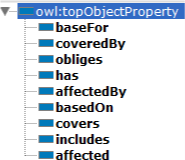
\includegraphics{object_props}
    \caption{Об'єктні параметри}
    \label{fig:object_props}
    \end{subfigure}
    \caption{Сутності онтології}
\end{figure}

Список створених об'єктів представлено на рисунку~\ref{fig:individuals}. Візуалізація розробленої онтології у вигляді графа представлена на рисунку~\ref{fig:ontograph}.

\begin{figure}[H]
	\centering
	    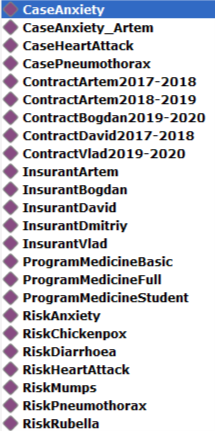
\includegraphics{individuals}
	\caption{Об'єкти}
	\label{fig:individuals}
\end{figure}

\begin{figure}[H]
	\centering
	    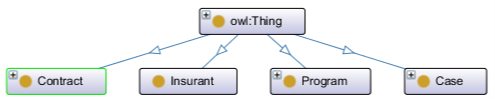
\includegraphics{ontograph}
	\caption{Графічна інтерпретація онтології}
	\label{fig:ontograph}
\end{figure}

\subsection{Запроси в Protege}
\subsubsection*{Запрос 1}
Перші 20 екземплярів класів та їх типи:
\lstinputlisting{code/sparql_1.txt} 

Результат виконання запросу зображений на рисунку~\ref{fig:sparql_1}.

\begin{figure}[H]
	\centering
	    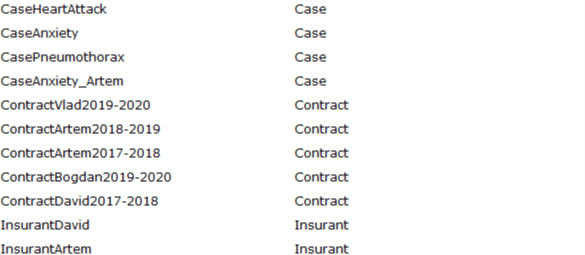
\includegraphics{sparql_1}
	\caption{Результат виконання запросу 1}
	\label{fig:sparql_1}
\end{figure}

\subsubsection*{Запрос 2}
Всі програми, по яким були виплати з початку 2018 року:
\lstinputlisting{code/sparql_2.txt} 

Результат виконання запросу зображений на рисунку~\ref{fig:sparql_2}.

\begin{figure}[H]
	\centering
	    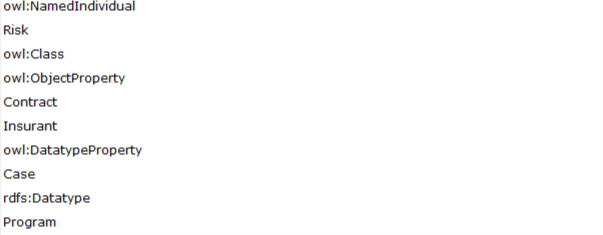
\includegraphics{sparql_2}
	\caption{Результат виконання запросу 2}
	\label{fig:sparql_2}
\end{figure}

\subsubsection*{Запрос 3}
Список \texttt{Insurant} з ім'ям <<Artem Chepurnoy>>:
\lstinputlisting{code/dl_1.txt} 

Результат виконання запросу зображений на рисунку~\ref{fig:dl_1}.

\begin{figure}[H]
	\centering
	    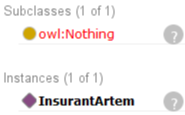
\includegraphics{dl_1}
	\caption{Результат виконання запросу 3}
	\label{fig:dl_1}
\end{figure}

\subsubsection*{Запрос 4}
Список \texttt{Program} які покривають ризик \texttt{RiskAnxiety}:
\lstinputlisting{code/dl_2.txt} 

Результат виконання запросу зображений на рисунку~\ref{fig:dl_2}.

\begin{figure}[H]
	\centering
	    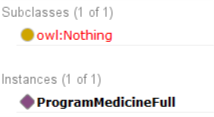
\includegraphics{dl_2}
	\caption{Результат виконання запросу 4}
	\label{fig:dl_2}
\end{figure}

\subsubsection*{Запрос 5}
Список \texttt{Contract} які покривають ризик \texttt{RiskPneumothorax}:
\lstinputlisting{code/dl_3.txt} 

Результат виконання запросу зображений на рисунку~\ref{fig:dl_3}.

\begin{figure}[H]
	\centering
	    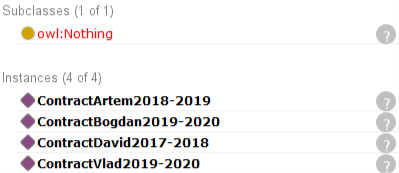
\includegraphics{dl_3}
	\caption{Результат виконання запросу 5}
	\label{fig:dl_3}
\end{figure}

\subsection{Розробка прототипу діагностичної експертної системи в CLIPS}
Факти предметної області:
\begin{enumerate}
	\item \textbf{income}: low, normal, high; 
	\item \textbf{age}: young, mature, elderly;
	\item \textbf{status}: single, plural.
\end{enumerate}

Правила предметної області:
\begin{enumerate}
	\item \textbf{income} high якщо >20000, normal якщо >10000, інакше low; 
	\item \textbf{age} elderly якщо >60, mature якщо >45, інакше young;
	\item \textbf{status} plural якщо є родина, інакше single.
	\item Правило результату приведено у вигляді таблиці: \\
		\begin{tabular}{l|lll}
			\textbf{Do I need an insurance?} & \textbf{income} & \textbf{age} & \textbf{status} \\\hline 
			\textbf{No} & low & young & single \\ 
			\textbf{No} & normal & young & single \\ 
			\textbf{Yes} & high & young & single \\ 
			\textbf{No} & low & mature & single \\ 
			\textbf{Yes} & normal & mature & single \\ 
			\textbf{Yes} & high & mature & single \\ 
			\textbf{Yes} & low & elderly & single \\ 
			\textbf{Yes} & normal & elderly & single \\ 
			\textbf{Yes} & high & elderly & single \\ 
			\textbf{No} & low & young & plural \\ 
			\textbf{Yes} & normal & young & plural \\ 
			\textbf{Yes} & high & young & plural \\ 
			\textbf{Yes} & low & mature & plural \\ 
			\textbf{Yes} & normal & mature & plural \\ 
			\textbf{Yes} & high & mature & plural \\ 
			\textbf{Yes} & low & elderly & plural \\ 
			\textbf{Yes} & normal & elderly & plural \\ 
			\textbf{Yes} & high & elderly & plural \\ 
		\end{tabular}
\end{enumerate}

Демонстрацію працездатності прототипа на конкретних прикладах представлено на рисунках~\ref{fig:test_1},~\ref{fig:test_2},~\ref{fig:test_3},~\ref{fig:test_4}.

\begin{figure}[H]
	\centering
	    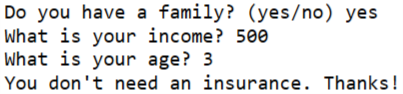
\includegraphics{test_1}
	\caption{Результат виконання програми №1}
	\label{fig:test_1}
\end{figure} 

\begin{figure}[H]
	\centering
	    
\includegraphics{test_2}
	\caption{Результат виконання програми №2}
	\label{fig:test_2}
\end{figure} 

\begin{figure}[H]
	\centering
	    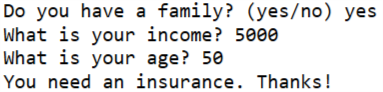
\includegraphics{test_3}
	\caption{Результат виконання програми №3}
	\label{fig:test_3}
\end{figure} 

\begin{figure}[H]
	\centering
	    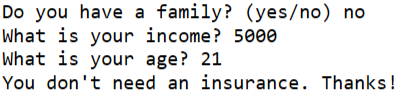
\includegraphics{test_4}
	\caption{Результат виконання програми №4}
	\label{fig:test_4}
\end{figure} 

Лістінг коду:
\lstinputlisting{code/main.clp} 

\subsection*{Висновки}
У ході виконання лабораторної роботи я сформував для ПО поле знань, список фактів, а також правил для роботи з ними. 
Також я оволодів базовими конструкціями мови представлення знань CLIPS, такими як deftemplate, deffacts, defrule, deffunction, defglobal. 
Я ознайомився з принципами пошуку рішення в експертних системах, заснованих на правилах виду "ЯКЩО-ТО", формування послідовності активації правил при виведенні результату.

\end{document}
